\chapter{Luca-Process}
	
Este capitulo describe el proceso de desarrollo e integración del componente gráfico (Process-Component). Se analizarán los aspectos del diseño y arquitectura a realizar así como las etapas de desarrollo del mismo.
	
\section{Arquitectura}

La arquitectura  de Luca-Process tras la integración del Process-Component, cambia ligera o mínimamente respecto a la arquitectura demostrada en la introducción. La siguiente figura describe la diferencia respecto a la figura anterior:

\begin{figure}[H]
	\centering
	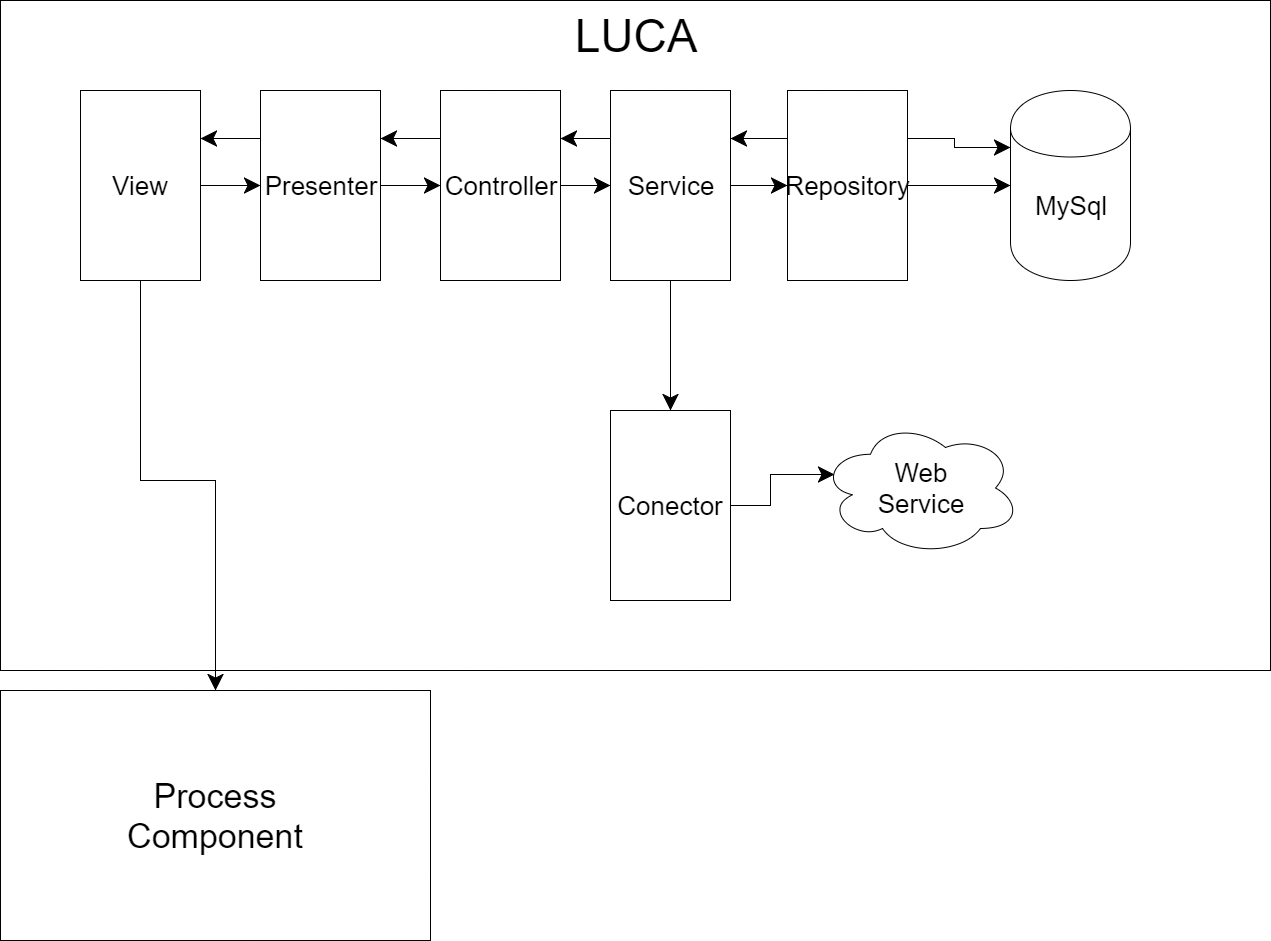
\includegraphics[scale=0.5]{arquitecturaLuca.png}
	\caption{Nueva Arquitectura de LUCA}\label{fig:arquitecturaLuca}
\end{figure}

Como se puede apreciar, la única diferencia reside en que en esta citada nueva funcionalidad se utiliza otro proyecto aparte, el cuál se encarga de forma exclusiva de proveer componentes de visualización para poder abordar la sintaxis de procesos y subprocesos que se enlazan entre sí mediante entradas y salidas.

\section{Desarrollo}

En esta sección se describe el proceso de desarrollo o implementación del componente de LUCA que integra el componente gráfico.

\vspace{5mm}

El primer paso para empezar a comprender el diseño y arquitectura de LUCA, fue realizar una pequeña prueba de concepto aplicando el patrón MVP\cite{mvp} e importando el componente gráfico para mostrar un proceso provisional, comprobando así el comportamiento del componente.


\vspace{5mm} 

Una vez comprobado el funcionamiento, se comienza la implementación por capas del proyecto, creando la capa controladora junto con sus anotaciones de seguridad, la capa de servicio que realiza llamadas a la capa de repositorio (implementada con Spring Data\cite{jpa}) para acceder a la base de datos, así como, al resto de servicios ya existentes en LUCA para la obtención de datos y ejecución de consultas. También se realizaron e implementaron, como se citó en la introducción, el conjunto de pruebas sobre la capa de servicio.

\vspace{5mm} 


Con las capas de datos implementadas


